\chapter{الأحماض والقواعد: Ka وpKa}\label{ch:g12:ka-and-pka}

كثير من النمل يدافع عن نفسه بحمض الميثانويك، وهو على الجلد
يحرق. وحمض الميثانويك \omterm{def:g11:functional-groups:carboxylic-acid}{حمض كربوكسيلي}
صغير. وحمض الهيدروكلوريك بالتركيز نفسه يحرق
أكثر بكثير. كلاهما حمض؛ وكلاهما يعطي \omterm{def:g2:mixing-and-dissolving:dissolve}{محلولًا} قيمة \omterm{def:g9:acids-bases-ph:ph}{pH} فيه أقل من 7؛ ومع ذلك
فليسا حمضيين بالطريقة نفسها. ولوصف حمض وصفًا كاملًا، يلزم
عددان: كم منه موجود، أي تركيزه، ومدى سهولة
تخليه عن \omterm{def:g9:ions:ion}{أيون} الهيدروجين، أي ثابت حمضيته.

\begin{recall}
المحاليل الحمضية والقاعدية والمتعادلة؛ وسلّم \omterm{def:g9:acids-bases-ph:ph}{pH}، من 0 إلى 14، الذي يكون أدنى
حين تكثر \omterm{def:g9:ions:ion}{أيونات} الهيدروجين (\cref{ch:g9:acids-bases-ph}).
\omterm{def:g12:equilibrium:quotient}{وخارج التفاعل} $Q$ \omterm{def:g12:equilibrium:constant}{وثابت التوازن} $K$
(\cref{ch:g12:equilibrium}). \omterm{def:g12:curly-arrows:curly-arrow}{والسهم المنحني} يبيّن حركة زوج من
\omterm{def:g9:inside-the-atom:nucleus}{الإلكترونات} (\cref{ch:g12:curly-arrows}).
\end{recall}

\begin{omfigure}
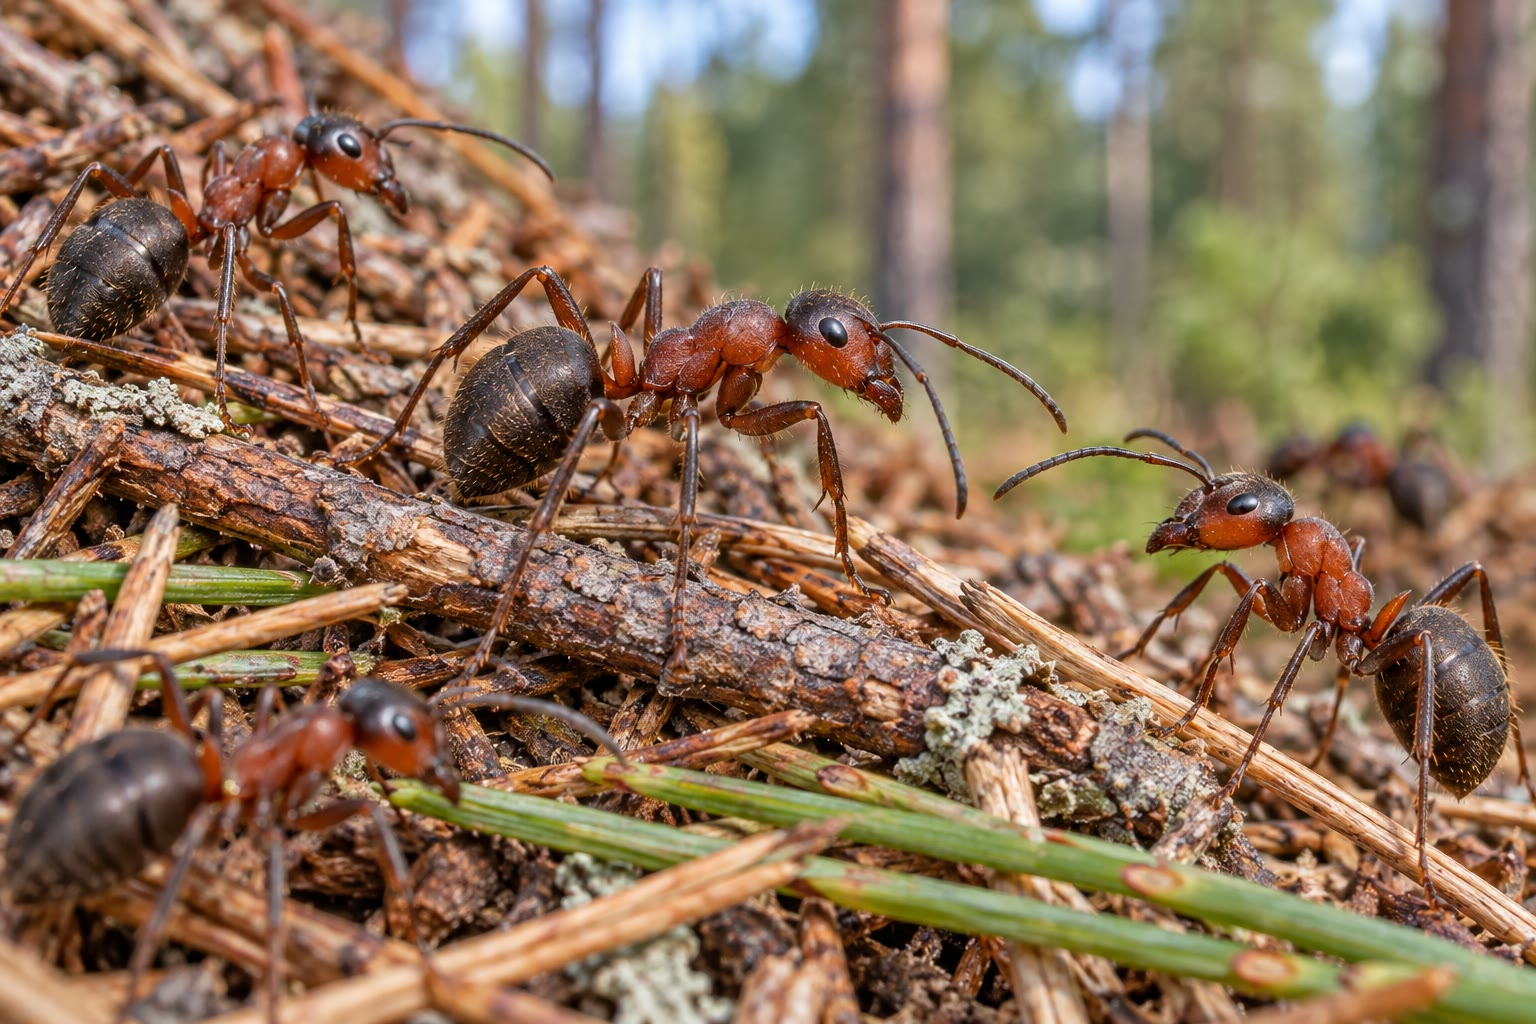
\includegraphics[width=0.45\linewidth]{images/book1/ai/g12-red-ants.jpg}

{\small نمل الغابات: كمثير من النمل، يدافع عن نفسه بحمض الميثانويك.}
\end{omfigure}

\section{أحماض برونستد وقواعده}

\begin{definition}[حمض برونستد وقاعدته، المزدوجة حمض/قاعدة]\label{def:g12:ka-and-pka:bronsted}
\emph{حمض برونستد}\index{حمض برونستد} \omterm{def:g6:pure-substances-and-mixtures:species}{نوع كيميائي} قادر على إعطاء
\omterm{def:g9:ions:ion}{أيون} هيدروجين \ce{H+}؛ و\emph{قاعدة برونستد}\index{قاعدة برونستد}
\omterm{def:g6:pure-substances-and-mixtures:species}{نوع كيميائي} قادر على أخذه. والحمض HA والقاعدة \ce{A-} التي يصير إليها
بفقد \ce{H+} يكوّنان \emph{مزدوجة حمض/قاعدة}\index{مزدوجة حمض/قاعدة}،
تُكتب $\ce{HA}/\ce{A-}$: $\ce{HA} \rightleftharpoons \ce{A-} + \ce{H+}$.
\end{definition}

\begin{definition}[أيون الأكسونيوم، الأمفوليت]\label{def:g12:ka-and-pka:oxonium}
في الماء لا يبقى \omterm{def:g9:ions:ion}{أيون} الهيدروجين وحده أبدًا: إذ يأخذه \omterm{def:g7:atoms-and-molecules:molecule}{جزيء}
ماء، فيعطي \emph{أيون الأكسونيوم}\index{أيون الأكسونيوم} \ce{H3O+}. \omterm{def:g6:pure-substances-and-mixtures:species}{والنوع
الكيميائي} الذي هو حمض مزدوجة وقاعدة مزدوجة أخرى
\emph{أمفوليت}\index{أمفوليت}؛ والماء أمفوليت، فهو حمض المزدوجة
$\ce{H2O}/\ce{OH-}$ وقاعدة المزدوجة $\ce{H3O+}/\ce{H2O}$.
\end{definition}

\begin{example}[حمض في الماء]\label{ex:g12:ka-and-pka:acid-water}
حين \omterm{def:g2:mixing-and-dissolving:dissolve}{يذوب} حمض الإيثانويك، يأخذ \omterm{def:g10:lewis-and-shape:lone-pair}{زوج حر} من \omterm{def:g7:atoms-and-molecules:molecule}{جزيء} ماء
هيدروجين الرابطة \ce{O-H} فيه، ويبقى زوج \ce{O-H} على أكسجين الحمض:
\[
  \ce{CH3COOH + H2O <=> CH3COO- + H3O+} .
\]
تتبادل مزدوجتان \omterm{def:g9:ions:ion}{أيون} هيدروجين: $\ce{CH3COOH}/\ce{CH3COO-}$ تعطيه،
و$\ce{H3O+}/\ce{H2O}$ تأخذه. ومن الآن فصاعدًا، تُكتب \omterm{def:g9:ions:ion}{أيونات} الهيدروجين في الفصول
السابقة \ce{H3O+} كلما كان الماء هو \omterm{def:g6:solutions-and-solubility:solute}{المذيب}.
\end{example}

\begin{omfigure}
\setchemfig{atom sep=2em}
\babelsublr{\chemfig{H_3C-C(=[2]O)-O-[@{oh}]@{h}H}\qquad
\chemfig{@{ow}\charge{90=\:,270=\:}{O}(-[:150]H)-[:210]H}
\qquad$\longrightarrow$\qquad
\chemfig{H_3C-C(=[2]O)-\charge{90=\:,0=\:,270=\:}{O}^{-}}\quad$+$\quad\ce{H3O+}}
\chemmove{
  \draw[->, thick, omProp, shorten <=4pt, shorten >=3pt]
    ($(ow)+(0,0.25)$) .. controls +(110:9mm) and +(60:9mm) .. (h);
  \draw[->, thick, omDef, shorten <=2pt, shorten >=4pt]
    (oh) .. controls +(-90:7mm) and +(-60:6mm) .. ($(oh)+(-0.3,-0.2)$);}

{\small ينتقل \omterm{def:g9:ions:ion}{أيون} هيدروجين من الحمض إلى الماء: \omterm{def:g10:lewis-and-shape:lone-pair}{زوج حر} من
الماء يكوّن الرابطة الجديدة \ce{O-H} (بالبرتقالي)، وزوج \ce{O-H} القديم
يبقى على أكسجين \omterm{def:g9:ions:ion}{أيون} الإيثانوات (بالأزرق).}
\end{omfigure}

\begin{history}[من أرهينيوس إلى برونستد، 1887--1923]
في سنة 1887 اقترح سفانته أرهينيوس أن الأحماض تعطي في الماء \omterm{def:g9:ions:ion}{أيونات} هيدروجين
وأن القواعد تعطي \omterm{def:g9:ions:ion}{أيونات} هيدروكسيد. وفي سنة 1923 وسّع يوهانس برونستد، ومستقلًا عنه
توماس لوري، الفكرة: فالحمض هو كل \omterm{def:g6:pure-substances-and-mixtures:species}{نوع كيميائي} يعطي
\omterm{def:g9:ions:ion}{أيون} هيدروجين، والقاعدة كل \omterm{def:g6:pure-substances-and-mixtures:species}{نوع كيميائي} يأخذه، في الماء أو في غيره. فصار
\omterm{def:g7:atoms-and-molecules:molecule}{جزيء} الأمونيا، الذي لا يحوي هيدروكسيدًا، قاعدة كأي قاعدة
أخرى.
\end{history}

\begin{omfigure}
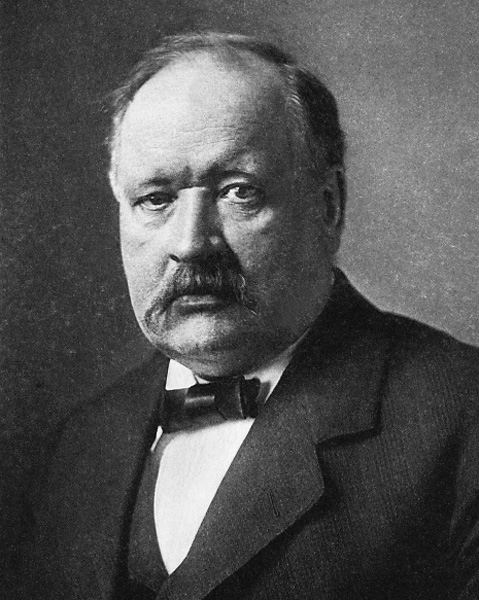
\includegraphics[width=0.22\linewidth]{images/book1/arrhenius.jpg}

{\small سفانته أرهينيوس (1859--1927).}
\end{omfigure}

\section{pH بلغة الأرقام}

\begin{definition}[pH، بدقة]\label{def:g12:ka-and-pka:ph-log}
في \omterm{def:g6:solutions-and-solubility:solute}{محلول مائي} مخفف، يُعرَّف \omterm{def:g9:acids-bases-ph:ph}{pH} بالعلاقة
\[
  \mathrm{pH} = -\log\frac{[\ce{H3O+}]}{c^\circ},
  \qquad\text{أي}\qquad
  [\ce{H3O+}] = c^\circ \times 10^{-\mathrm{pH}} ,
\]
حيث $\log$ اللوغاريتم العشري.
\end{definition}

\begin{proposition}[التخفيف عشر مرات، وحدة واحدة]\label{prop:g12:ka-and-pka:dilution}
إذا قُسم $[\ce{H3O+}]$ على 10، زادت قيمة \omterm{def:g9:acids-bases-ph:ph}{pH} بواحد؛ وإذا
ضُرب في 10، نقصت بواحد.
\end{proposition}

\begin{proof}
$-\log\big([\ce{H3O+}]/10c^\circ\big) = -\log\big([\ce{H3O+}]/c^\circ\big)
+ \log 10 = \mathrm{pH} + 1$.
\end{proof}

\begin{definition}[الأحماض والقواعد القوية والضعيفة]\label{def:g12:ka-and-pka:strong-acid}
\emph{الحمض القوي}\index{حمض قوي} يتفاعل مع الماء \omterm{def:g10:reaction-progress-table:limiting}{تفاعلًا تامًا}: فلا يبقى شيء
من الحمض على حاله في \omterm{def:g2:mixing-and-dissolving:dissolve}{المحلول}. و\emph{الحمض
الضعيف}\index{حمض ضعيف} يتفاعل جزئيًا: فتفاعله مع الماء يبلغ
توازنًا. وكذلك \emph{القاعدة القوية}\index{قاعدة قوية} تتفاعل
مع الماء \omterm{def:g10:reaction-progress-table:limiting}{تفاعلًا تامًا}، و\emph{القاعدة الضعيفة}\index{قاعدة ضعيفة} جزئيًا.
\end{definition}

\begin{proposition}[pH حمض قوي]\label{prop:g12:ka-and-pka:strong}
\omterm{def:g2:mixing-and-dissolving:dissolve}{لمحلول} \omterm{def:g12:ka-and-pka:strong-acid}{حمض قوي} تركيزه $c$ (غير مخفف جدًا)
$[\ce{H3O+}] = c$ و$\mathrm{pH} = -\log(c/c^\circ)$.
\end{proposition}

\begin{proof}
التفاعل \ce{HA + H2O -> A- + H3O+} تام: فكل \omterm{def:g7:atoms-and-molecules:molecule}{جزيء} من الحمض
يعطي \omterm{def:g9:ions:ion}{أيون} أكسونيوم واحدًا. \omterm{def:g9:ions:ion}{والأيونات} الآتية من الماء نفسه مهملة
ما دام $c$ أكبر بكثير من \qty{e-7}{mol/L}.
\end{proof}

\begin{example}[حمض الهيدروكلوريك]\label{ex:g12:ka-and-pka:hcl}
حمض الهيدروكلوريك بتركيز \qty{0.010}{mol/L}: $[\ce{H3O+}] = \qty{0.010}{mol/L}$
و$\mathrm{pH} = -\log 0.010 = 2.0$. وإذا خُفف عشر مرات، صارت \omterm{def:g9:acids-bases-ph:ph}{pH} 3.0.
\end{example}

\section{الماء والجداء الأيوني}


\begin{definition}[الجداء الأيوني للماء]\label{def:g12:ka-and-pka:ionic-product}
يتفاعل الماء تفاعلًا طفيفًا جدًا مع نفسه، \ce{2H2O <=> H3O+ + OH-}. وثابت
توازن هذا التفاعل هو \emph{الجداء الأيوني
للماء}\index{الجداء الأيوني للماء}:
\[
  K_e = \frac{[\ce{H3O+}]\,[\ce{OH-}]}{(c^\circ)^2},
  \qquad pK_e = -\log K_e .
\]
\end{definition}

\begin{proposition}[الماء المتعادل والقواعد القوية]\label{prop:g12:ka-and-pka:ke}
% ledger: ke:25C
عند \qty{25}{\celsius}، $K_e = \num{1.0e-14}$ و$pK_e = 14.0$. وفي الماء
النقي $[\ce{H3O+}] = [\ce{OH-}] = \qty{1.0e-7}{mol/L}$: أي \omterm{def:g9:acids-bases-ph:ph}{pH} 7.0. \omterm{def:g12:ka-and-pka:strong-acid}{وقاعدة
قوية} تركيزها $c$ تعطي $[\ce{OH-}] = c$، إذن
$[\ce{H3O+}] = K_e (c^\circ)^2 / c$ و$\mathrm{pH} = 14.0 + \log(c/c^\circ)$.
\end{proposition}

\begin{proof}
في الماء النقي يأتي الأيونان أزواجًا، فهما متساويان،
وجداؤهما $\num{1.0e-14}$: فكل منهما \qty{1.0e-7}{mol/L}. وللقاعدة،
يبقى $K_e$ صالحًا في \omterm{def:g2:mixing-and-dissolving:dissolve}{المحلول}:
$-\log([\ce{H3O+}]/c^\circ) = -\log K_e + \log(c/c^\circ)$.
\end{proof}

\begin{example}[هيدروكسيد الصوديوم]\label{ex:g12:ka-and-pka:naoh}
هيدروكسيد الصوديوم بتركيز \qty{0.010}{mol/L}: $[\ce{OH-}] = 0.010$، إذن
$[\ce{H3O+}] = \num{1.0e-14}/0.010 = \qty{1.0e-12}{mol/L}$ \omterm{def:g9:acids-bases-ph:ph}{وpH} 12.0.
\end{example}

\section{ثابت الحمضية}

\begin{definition}[ثابت الحمضية، $pK_a$]\label{def:g12:ka-and-pka:ka}
\emph{ثابت الحمضية}\index{ثابت الحمضية} $K_a$ لمزدوجة
$\ce{HA}/\ce{A-}$ هو ثابت توازن تفاعل الحمض
مع الماء، \ce{HA + H2O <=> A- + H3O+}:
\[
  K_a = \frac{[\ce{A-}]\,[\ce{H3O+}]}{[\ce{HA}]\,c^\circ} .
\]
و\emph{pKa}\index{pKa} المزدوجة هو
$pK_a = -\log K_a$.
\end{definition}

\begin{proposition}[كلما صغر $pK_a$، قوي الحمض]\label{prop:g12:ka-and-pka:compare}
من بين حمضين ضعيفين بالتركيز نفسه، يتفاعل مع الماء أكثر، ويعطي
\omterm{def:g9:acids-bases-ph:ph}{pH} أدنى، الحمضُ الذي له $K_a$ أكبر، أي $pK_a$ أصغر؛
وقاعدته المرافقة هي الأضعف.
\end{proposition}

\begin{proof}
$K_a$ الأكبر يعني مزيدًا من \ce{A-} و\ce{H3O+} عند التوازن للكمية
نفسها من \ce{HA}. وقاعدة المزدوجة \ce{A-} التي يتخلى حمضها عن \omterm{def:g9:ions:ion}{أيون} الهيدروجين
بسهولة تستعيده على مضض.
\end{proof}

\begin{omfigure}
\begin{tikzpicture}[font=\small, y=0.55cm]
  % ledger: pka:methanoic, pka:ethanoic, pka:benzoic, pka:ascorbic1, ka:HF, ka:H2CO3, ka:HCO3, kb:NH3, ke:25C
  \draw[->, thick] (0,0) -- (0,14.8) node[above] {$pK_a$};
  \foreach \k in {0,2,4,6,8,10,12,14} \draw (-0.1,\k) -- (0.1,\k) node[right, font=\scriptsize] {\k};
  \node[font=\footnotesize\bfseries, anchor=south] at (-3.0,14.3) {الحمض};
  \node[font=\footnotesize\bfseries, anchor=south] at (3.0,14.3) {القاعدة};
  \foreach \p/\yl/\acid/\base in {3.19/2.9/{\ce{HF}}/{\ce{F-}},
      3.74/3.6/{\ce{HCOOH}}/{\ce{HCOO-}}, 4.04/4.3/{حمض الأسكوربيك}/{الأسكوربات},
      4.20/5.0/{\ce{C6H5COOH}}/{\ce{C6H5COO-}}, 4.76/5.7/{\ce{CH3COOH}}/{\ce{CH3COO-}},
      6.37/6.9/{\ce{CO2,H2O}}/{\ce{HCO3-}}, 9.26/9.26/{\ce{NH4+}}/{\ce{NH3}},
      10.33/10.4/{\ce{HCO3-}}/{\ce{CO3^{2-}}}} {
    \draw[omDef] (-0.25,\p) -- (0.25,\p);
    \draw[black!40] (-0.25,\p) -- (-1.1,\yl);
    \draw[black!40] (0.25,\p) -- (1.1,\yl);
    \node[anchor=east, font=\scriptsize] at (-1.15,\yl) {\acid};
    \node[anchor=west, font=\scriptsize] at (1.15,\yl) {\base};
  }
  \draw[->, omThm, thick] (-4.6,13) -- (-4.6,1);
  \node[omThm, rotate=90, font=\footnotesize] at (-4.95,7) {أحماض أقوى};
  \draw[->, omMeth, thick] (4.6,1) -- (4.6,13);
  \node[omMeth, rotate=90, font=\footnotesize] at (4.95,7) {قواعد أقوى};
\end{tikzpicture}

{\small بعض المزدوجات مرتبة بحسب $pK_a$ عند \qty{25}{\celsius}، الأحماض
على اليسار، وقواعدها على اليمين. كلما انخفضت المزدوجة على السلّم،
قوي حمضها؛ وكلما ارتفعت، قويت قاعدتها.}
\end{omfigure}


\begin{method}[pH حمض ضعيف]\label{met:g12:ka-and-pka:weak}
\omterm{def:g12:ka-and-pka:strong-acid}{لحمض ضعيف} تركيزه $c$ وثابته $K_a$:
\begin{enumerate}
  \item اكتب جدول \omterm{def:g10:reaction-progress-table:extent}{تقدم التفاعل} \ce{HA + H2O <=> A- + H3O+} لكل لتر،
        مع $x = [\ce{H3O+}]$: $[\ce{HA}] = c - x$، $[\ce{A-}] = x$
        (بإهمال \omterm{def:g9:ions:ion}{أيونات} الماء نفسه).
  \item حلّ $\dfrac{x^2}{(c - x)\,c^\circ} = K_a$، أي المعادلة من الدرجة الثانية
        $x^2 + K_a c^\circ x - K_a c^\circ c = 0$، محتفظًا بالجذر
        الموجب.
  \item $\mathrm{pH} = -\log(x/c^\circ)$؛ وتحقق من أن $x$ أكبر بكثير
        من \qty{e-7}{mol/L}.
\end{enumerate}
\end{method}

\begin{example}[حمض الإيثانويك بتركيز \texorpdfstring{\qty{0.010}{mol/L}}{0.010 mol/L}]\label{ex:g12:ka-and-pka:acetic}
% ledger: pka:ethanoic
$pK_a = 4.76$، إذن $K_a = 10^{-4.76} = \num{1.74e-5}$. ثم إن
$x^2 + \num{1.74e-5}\,x - \num{1.74e-7} = 0$ تعطي
$x = \qty{4.1e-4}{mol/L}$ \omterm{def:g9:acids-bases-ph:ph}{وpH} 3.39. فلم يتفاعل مع الماء إلا $\num{4.1e-4}/0.010 =
\qty{4.1}{\percent}$ من الحمض؛ أما حمض الهيدروكلوريك
بالتركيز نفسه، \omterm{def:g9:acids-bases-ph:ph}{وpH} له 2.0، فقد تفاعل كله.
\end{example}

\begin{omfigure}
\begin{tikzpicture}[font=\small]
  \fill[omThm!45] (0,1.3) rectangle (8,2.0);
  \node[anchor=east] at (-0.1,1.65) {\ce{HCl}, \qty{0.010}{mol/L}};
  \node[white, font=\small\bfseries] at (4,1.65) {\ce{H3O+} + \ce{Cl-}: \qty{100}{\percent}};
  \fill[omDef!35] (0,0) rectangle (7.67,0.7);
  \fill[omThm!45] (7.67,0) rectangle (8,0.7);
  \node[anchor=east] at (-0.1,0.35) {\ce{CH3COOH}, \qty{0.010}{mol/L}};
  \node at (3.8,0.35) {\foreignlanguage{arabic}{\ce{CH3COOH} الباقي على حاله: \qty{95.9}{\percent}}};
  \draw[<-, omThm] (7.85,0.75) -- (8.4,1.1) node[right, font=\footnotesize] {\foreignlanguage{arabic}{\qty{4.1}{\percent} متأيّن}};
\end{tikzpicture}

{\small ما يؤول إليه \omterm{def:g12:ka-and-pka:strong-acid}{حمض قوي} \omterm{def:g12:ka-and-pka:strong-acid}{وحمض ضعيف} بالتركيز
نفسه: \omterm{def:g12:ka-and-pka:strong-acid}{الحمض القوي} يتحول كله إلى \omterm{def:g9:ions:ion}{أيونات}، \omterm{def:g12:ka-and-pka:strong-acid}{والحمض الضعيف}
لا يكاد يتحول. ومن هنا الفرق في \omterm{def:g9:acids-bases-ph:ph}{pH}، 2.0 مقابل 3.4.}
\end{omfigure}

\begin{safety}{\ghs[0.75cm]{GHS02}\ghs[0.75cm]{GHS05}\ghs[0.75cm]{GHS06}\ghs[0.75cm]{GHS07}}
% ledger: ghs:formic-acid
حمض الميثانويك المركّز قابل للاشتعال، ويسبب حروقًا شديدة للجلد
والعينين، وبخاره سام. ولا يتناوله إلا المعلم،
تحت ساحبة الأبخرة؛ أما المحاليل المخففة في التمارين فتحتاج هي أيضًا إلى
نظارتين واقيتين.
\end{safety}

\section{تمارين}

\begin{exercise}[$\star$]\label{exo:g12:ka-and-pka:1}
أعطِ القاعدة المرافقة لكل من: \ce{HCOOH}، \ce{NH4+}، \ce{H2O}، \ce{HCO3-}؛
والحمض المرافق لكل من: \ce{NH3}، \ce{OH-}، \ce{H2O}، \ce{HCO3-}.
وأي الأنواع أمفوليتات؟
\end{exercise}

\begin{exercise}[$\star$]\label{exo:g12:ka-and-pka:2}
احسب \omterm{def:g9:acids-bases-ph:ph}{pH} حمض الهيدروكلوريك بالتراكيز \qty{0.10}{mol/L}،
و\qty{0.0010}{mol/L} و\qty{5.0e-3}{mol/L}.
\end{exercise}

\begin{exercise}[$\star$]\label{exo:g12:ka-and-pka:3}
\omterm{def:g2:mixing-and-dissolving:dissolve}{لمحلول} \omterm{def:g9:acids-bases-ph:ph}{pH} قيمتها 4.5. احسب $[\ce{H3O+}]$. ولمحلول \omterm{def:g9:acids-bases-ph:ph}{pH} قيمتها 11.2:
احسب $[\ce{H3O+}]$ و$[\ce{OH-}]$ عند \qty{25}{\celsius}.
\end{exercise}

\begin{exercise}[$\star$]\label{exo:g12:ka-and-pka:4}
اكتب التفاعل مع الماء وعبارة $K_a$ لحمض
الميثانويك ولأيون الأمونيوم.
\end{exercise}

\begin{exercise}[$\star$]\label{exo:g12:ka-and-pka:5}
أيهما الحمض الأقوى: حمض الميثانويك ($pK_a = 3.74$) أم حمض
الإيثانويك ($pK_a = 4.76$)؟ وأيهما القاعدة الأقوى: \ce{HCOO-} أم
\ce{CH3COO-}؟
\end{exercise}

\begin{exercise}[$\star\star$]\label{exo:g12:ka-and-pka:6}
\omterm{def:g2:mixing-and-dissolving:dissolve}{لمحلول} \omterm{def:g12:ka-and-pka:strong-acid}{حمض ضعيف} HA بتركيز \qty{0.050}{mol/L} \omterm{def:g9:acids-bases-ph:ph}{pH} قيمتها 3.0. احسب
$[\ce{A-}]$ و$[\ce{HA}]$، ثم $K_a$ و$pK_a$.
\end{exercise}

\begin{exercise}[$\star\star$]\label{exo:g12:ka-and-pka:7}
احسب \omterm{def:g9:acids-bases-ph:ph}{pH} حمض البنزويك بتركيز \qty{0.020}{mol/L} ($pK_a = 4.20$).
\end{exercise}

\begin{exercise}[$\star\star$]\label{exo:g12:ka-and-pka:8}
احسب \omterm{def:g9:acids-bases-ph:ph}{pH} \omterm{def:g2:mixing-and-dissolving:dissolve}{محلول} هيدروكسيد الصوديوم بتركيز \qty{2.0e-3}{mol/L}.
\end{exercise}

\begin{exercise}[$\star\star$]\label{exo:g12:ka-and-pka:9}
مستعينًا بسلّم $pK_a$، رتّب أحماض المزدوجات المبيّنة من
الأقوى إلى الأضعف. وأين يقع \omterm{def:g12:ka-and-pka:strong-acid}{حمض قوي} مثل \ce{HCl}؟
\end{exercise}

\begin{exercise}[$\star\star$]\label{exo:g12:ka-and-pka:10}
ثنائي أكسيد الكربون \omterm{def:g6:solutions-and-solubility:solute}{المذاب} في الماء يجعله حمضيًا قليلًا (المزدوجة
$\ce{CO2,H2O}/\ce{HCO3-}$، $pK_a = 6.37$). ووُجد أن عيّنة من ماء المطر الملامس
\omterm{def:g4:air-a-mixture-of-gases:air}{للهواء} قيمة \omterm{def:g9:acids-bases-ph:ph}{pH} فيها 5.6. احسب $[\ce{H3O+}]$، وقارن بالماء النقي.
\end{exercise}

\begin{exercise}[$\star\star$]\label{exo:g12:ka-and-pka:11}
بيّن أنه للمزدوجة $\ce{NH4+}/\ce{NH3}$، $pK_a = pK_e - pK_b$، حيث
$K_b = \num{1.8e-5}$ ثابت التفاعل \ce{NH3 + H2O <=> NH4+ + OH-}.
واحسب $pK_a$.
\end{exercise}

\begin{exercise}[$\star\star\star$]\label{exo:g12:ka-and-pka:12}
لحمض الإيثانويك بتركيز \qty{0.010}{mol/L} قيمة \omterm{def:g9:acids-bases-ph:ph}{pH} تساوي 3.39. احسب \omterm{def:g9:acids-bases-ph:ph}{pH} بعد
تخفيفه عشر مرات. أترتفع بوحدة واحدة، كما في حالة \omterm{def:g12:ka-and-pka:strong-acid}{الحمض القوي}؟
اشرح.
\end{exercise}

\begin{exercise}[$\star\star\star$]\label{exo:g12:ka-and-pka:13}
\omterm{def:g9:ions:ion}{أيون} الهيدروجينوكربونات \omterm{def:g12:ka-and-pka:oxonium}{أمفوليت}. اكتب تفاعليه مع
الماء وثابتيهما، مستعينًا بسلّم $pK_a$. أيهما أكبر؟
وماذا يوحي ذلك بشأن \omterm{def:g9:acids-bases-ph:ph}{pH} \omterm{def:g2:mixing-and-dissolving:dissolve}{محلول} هيدروجينوكربونات
الصوديوم؟
\end{exercise}

\begin{exercise}[$\star\star\star$]\label{exo:g12:ka-and-pka:14}
يُخفَّف حمض الهيدروكلوريك ذو التركيز \qty{1.0e-3}{mol/L} ألف مرة،
ثم ألف مرة أخرى. فتعطي قاعدة متسرّعة \omterm{def:g9:acids-bases-ph:ph}{pH} 6، ثم \omterm{def:g9:acids-bases-ph:ph}{pH} 9. لماذا
تستحيل \omterm{def:g9:acids-bases-ph:ph}{pH} 9 لحمض مخفف؟ ومن أي قيمة تقترب \omterm{def:g9:acids-bases-ph:ph}{pH} \omterm{def:g2:mixing-and-dissolving:dissolve}{المحلول}
الشديد \omterm{def:g10:concentration-and-dilution:dilution}{التخفيف}؟
\end{exercise}

\begin{exercise}[$\star\star\star$]\label{exo:g12:ka-and-pka:15}
حمض الأسكوربيك (فيتامين C، $pK_a = 4.04$، $M = \qty{176.0}{g/mol}$): يُذاب
قرص كتلته \qty{500}{mg} في \qty{200}{mL} من الماء. احسب
\omterm{def:g9:acids-bases-ph:ph}{pH} (مقتصرًا على الحمضية الأولى).
\end{exercise}

\section{مسألة: سمّ النملة}


\begin{problem}[{مسألة نهاية الأسبوع --- ما pH محلول حمض الميثانويك في سمّ
النملة بتركيز 0.010 mol/L، وكيف تسكّن صودا الخبز لسعته؟}]
\label{pb:g12:ka-and-pka:1}
% ledger: src:formic-ants, pka:methanoic, ka:H2CO3, ke:25C, aw:C, aw:H, aw:O
يوجد حمض الميثانويك، \ce{HCOOH}، في سمّ النمل. وقيمة $pK_a$ له عند
\qty{25}{\celsius} هي 3.74. ندرس \omterm{def:g2:mixing-and-dissolving:dissolve}{محلولًا} منه بتركيز \qty{0.010}{mol/L}
ونقارنه بحمض الهيدروكلوريك.

\medskip
\noindent\textbf{الجزء الأول --- الحمض.}
\begin{enumerate}
  \item ارسم صيغة لويس لحمض الميثانويك وأحط بدائرة
        الهيدروجين الذي يعطيه.
  \item اكتب مزدوجته وتفاعله مع الماء.
  \item اكتب $K_a$ واحسب قيمته.
  \item ضع المزدوجة على سلّم $pK_a$: أحمض الميثانويك أقوى
        من حمض الإيثانويك أم أضعف؟
  \item احسب كتلة حمض الميثانويك في \qty{1.0}{L} من
        \omterm{def:g2:mixing-and-dissolving:dissolve}{المحلول}.
\end{enumerate}

\medskip
\noindent\textbf{الجزء الثاني --- \omterm{def:g9:acids-bases-ph:ph}{pH}.}
\begin{enumerate}[resume]
  \item املأ \omterm{def:g10:reaction-progress-table:extent}{جدول التقدم} لكل لتر، مع $x = [\ce{H3O+}]$.
  \item اكتب المعادلة $Q_{eq} = K_a$.
  \item حلّها.
  \item احسب \omterm{def:g9:acids-bases-ph:ph}{pH}.
  \item ما الكسر الذي تفاعل مع الماء من الحمض؟
  \item تحقق من أن \omterm{def:g9:ions:ion}{الأيونات} الآتية من الماء يمكن إهمالها.
\end{enumerate}

\medskip
\noindent\textbf{الجزء الثالث --- مقارنة.}
\begin{enumerate}[resume]
  \item ما \omterm{def:g9:acids-bases-ph:ph}{pH} حمض الهيدروكلوريك بتركيز \qty{0.010}{mol/L}؟
  \item كم مرة يزيد ما يحويه من \omterm{def:g9:ions:ion}{أيونات} الأكسونيوم على ما يحويه
        \omterm{def:g2:mixing-and-dissolving:dissolve}{محلول} حمض الميثانويك؟
  \item اشرح الفرق، مستعملًا كلمتي قوي وضعيف.
\end{enumerate}

\medskip
\noindent\textbf{الجزء الرابع --- صودا الخبز.}
\begin{enumerate}[resume]
  \item صودا الخبز هي هيدروجينوكربونات الصوديوم. اكتب التفاعل
        بين حمض الميثانويك \omterm{def:g9:ions:ion}{وأيون} الهيدروجينوكربونات (وهو يعطي
        الميثانوات و\ce{CO2,H2O}).
  \item بيّن أن ثابته $K = K_a(\ce{HCOOH}) / K_a(\ce{CO2,H2O})$،
        واحسبه.
  \item أهذا التفاعل ملائم؟ وأي غاز يُرى؟
  \item لماذا تُفضَّل على الجلد قاعدة أضعف بكثير من الهيدروكسيد، كالهيدروجينوكربونات؟
  \item اذكر الجواب النهائي: ما \omterm{def:g9:acids-bases-ph:ph}{pH} \omterm{def:g2:mixing-and-dissolving:dissolve}{محلول} حمض الميثانويك
        بتركيز \qty{0.010}{mol/L}؟
\end{enumerate}
\end{problem}
